\documentclass{article}
\usepackage[utf8]{inputenc}
\usepackage{fullpage}
\usepackage{amsmath}
\usepackage{verbatim}
\usepackage{graphicx}
\usepackage{hyperref}
\hypersetup{colorlinks=true,linktoc=all}
\usepackage{listing}
\usepackage{subcaption}
\usepackage[table]{xcolor}
\usepackage{multirow}
\usepackage{cleveref}
\usepackage{xspace}

\newcommand{\filter}{\textit{Filter}\xspace}
\newcommand{\projection}{\textit{Projection}\xspace}
\newcommand{\join}{\textit{Join}\xspace}
\newcommand{\sort}{\textit{Sort}\xspace}
\newcommand{\indexing}{\textit{Indexing}\xspace}
\newcommand{\groupby}{\textit{Group By}\xspace}
\newcommand{\topk}{\textit{TopK}\xspace}


\title{In-Storage SQL Processing\\
  \large MIT CSAIL Joint Research Proposal} \author{Shuotao Xu, Xiangyao Yu\\
  CSG Group, DB Group\\
  (shuotao@csail.mit.edu), (yxy@csail.mit.edu)}

\begin{document}
\maketitle
\section{Introduction}
With the ever-growing data size for big data applications, technology for fast and efficient data storage and computation is becoming increasingly crucial for supporting complex queries on large datasets.
For big-data applications, a large number of analytic platforms rely on relational database systems, such as MySQL and Postgres, to store large datasets and running complex SQL queries.

Many databases are running in the cloud due to its high elasticity and lower cost, examples including Presto~\cite{presto}, Redshift~\cite{redshift}, and Snowflake~\cite{snowflake}.
In today's cloud, storage and compute are typically decoupled on different physical servers, such as Amazon's AWS Cloud~\cite{aws} and Microsoft's Azure Cloud~\cite{azure}. 
Separation of compute and storage simplifies the management of data and improves elasticity. 
To perform data analytics on such clouds, however, a database system needs to bring data from flash disk on the storage node via the interconnecting network to the CPU cache of the compute node to perform analysis of the fetched data.
As the network bandwidth (e.g., 10 Gigabit Ethernet) is typically lower than the IO bandwidth at the storage nodes (e.g., up to 16~GB/s for i3 instance in AWS), the network can become a significant bottleneck for query processing. 
% SQL query processing, since the network I/O bandwidth can be much slower than aggregate bandwidth of the flash disks on storage node.

The bandwidth imbalance between the network and the disks also exists in SQL processing on a single node server.
Like distributed SQL processing, a processor loads data from flash disks via PCIe bus to the CPU cache to perform SQL analysis on a single node.
A flash disk is typically connected to the processor via 4 lanes of PCIe gen3 bus, which provide a bandwidth of 4GB/s.
The flash chips inside a flash disk, however, can provide internal aggregate bandwidth that is much greater than the PCIe gen3 bus, if they are organized in a parallel architecture~\cite{biscuit, guz-systor17}.
Therefore, the communication channel between the processor and the disks can also be a bottleneck in a single node setting. 

In today's flash storage technology development, both industry and academia are trying to enable Near-Data Processing (NDP) capabilities, such as ARM processors and FPGAs, to application developers~\cite{biscuit, ibex, bluedbm, netezza, exadata, jafar, do2013query, sukhwani2012database, fpga-sort}.
In this research, we want to investigate how to use such in-storage computation to offload some of the SQL operators inside flash drives to boost SQL query performance on both a single servers and a cluster of servers.
We propose to investigate seven important SQL operators for the benefit of in-storage processing: \filter, \projection, \join, \sort, \indexing, \groupby, and \topk.
We will devise new techniques to implement these operators on the computation devices (e.g., ARM-based processor or FPGA) inside the storage, which may have limited computation power and memory size. 
For this project, we mainly focus on IO-intensive operators such as \filter, \projection, \join, \sort, \groupby and \topk and investigate how NDP can reduce the amount of IO traffic for these operators. 
For now, we do not study operators (e.g., \sort) that do not saturate the IO bandwidth. 

Specifically, the proposed research will make the following contributions.

\begin{itemize}
\item We extensively study seven widely used operators in SQL-based relational databases. For each operator, we conduct a qualitative analysis of whether it can benefit from near-data processing. 

\item For each operator, we propose a design that partition the operator's functionality between the host node and the storage node to reduce the amount of IO traffic and CPU computation time. 

\item We incorporate the design into an open-source database (e.g., MySQL or SQLite) and evaluate the performance advantage of each design we propose, compared to a non-NDP database. 
\end{itemize}

Please note that this MIT internal collaboration between Computer Structure Group and Database Group has started prior to the Samsung Internship. We will pursue this research in an open-source domain.

\section{System Architecture}

A relational query processor takes a declarative SQL statement, validates it, optimizes it into a procedural dataflow execution plan, and executes that dataflow program on behalf of a user.
A relational query processor typically has four major software components 1) Query Parser, 2) Query Rewriter, 3) Query Optimizer, and 4) Plan Executor.
The first three components generate a query plan. The Plan Executor issues disk IOs to the storage device which executes the plan as shown in Figure~\ref{fig:software}.

In this proposal, we will split the functionality of the Plan Executor between the host server and the near-data processors which can be ARM processors, or FPGAs, or both. 
The communication channel is implemented using RPCs and DMAs over PCIe or Ethernet.
Via this channel, IO-intensive operations can be sent to the near-data processor on the flash drive, as shown in Figure~\ref{fig:accelerator}.
The functionalities pushed down to the near-data processor are simple and consume only limited computation power and memory space. 
Yet, the near-data processor can utilize the entire aggregate internal NAND flash bandwidth, while reducing the IO traffic to the compute node. 

\begin{figure}[!htb]
  \centering
    \begin{subfigure}[t]{0.40\textwidth}
      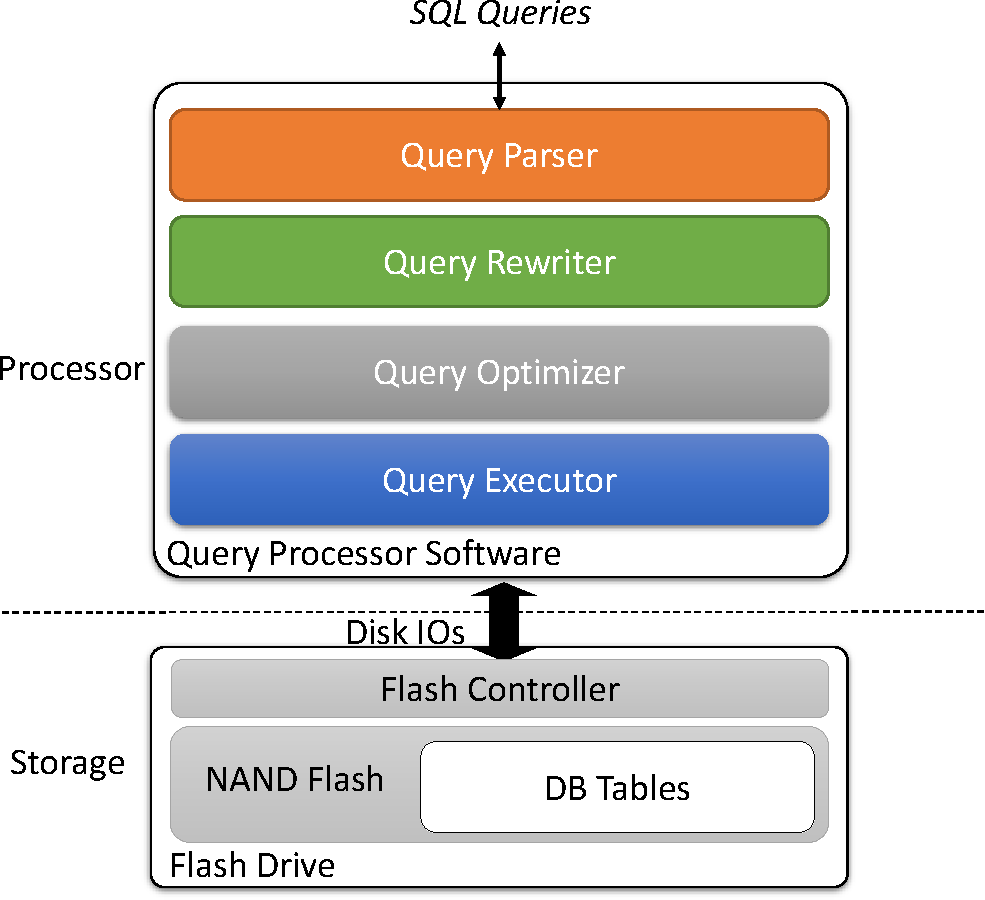
\includegraphics[width=\textwidth]{figures/software-stack-crop.pdf}
      \caption{Traditional SQL Query processing stack}
      \label{fig:software}
  \end{subfigure}\hspace{50pt}
  \begin{subfigure}[t]{0.40\textwidth}
    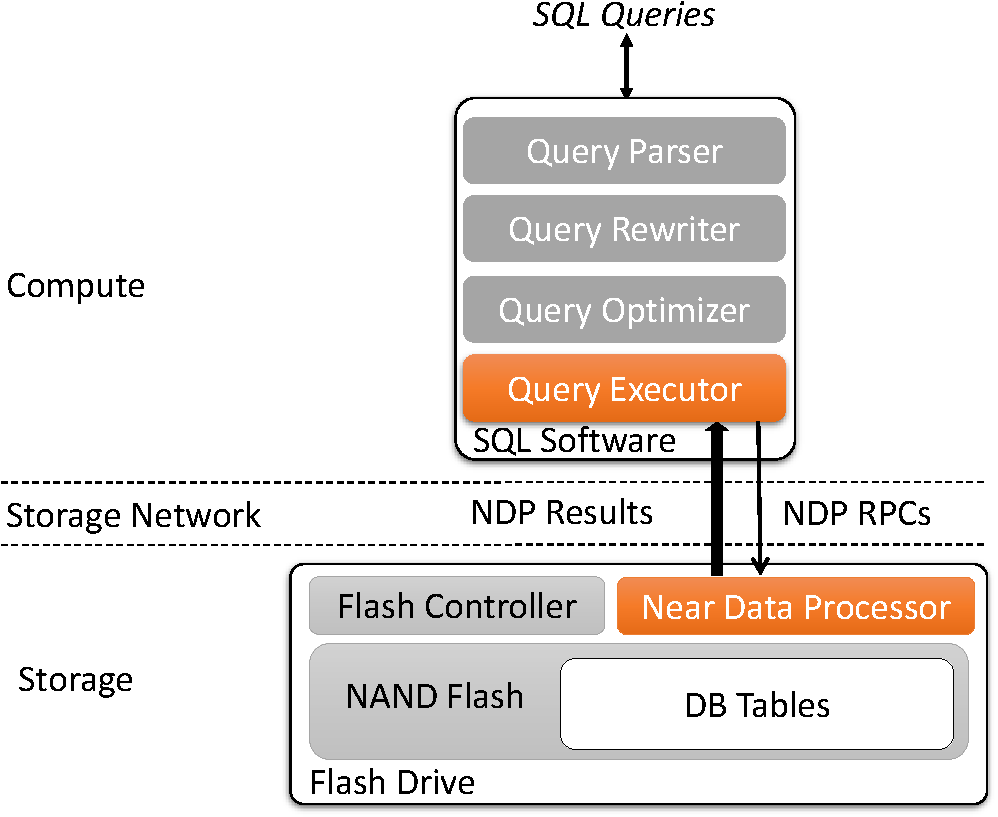
\includegraphics[width=\textwidth]{figures/accelerator-stack-crop.pdf}
    \caption{SQL Query processing stack with near-storage processor}
    \label{fig:accelerator}
  \end{subfigure}
  \label{fig:try}
  \caption{DBMS Query Processing Architectures}
\end{figure}

\section{SQL Operators}

In this section, we qualitatively investigate seven most commonly used operators in a database and discusses whether they are amenable to near-data processing (\cref{sec:analysis}). Then, we discuss how each individual operators can be performed using NDP from Section~\ref{sec:join} to \ref{sec:index}.

\subsection{Qualitative Analysis of Operators} \label{sec:analysis}

Table~\ref{tab:operators} presents the seven operators that we focus on. For each operator, we present the average time complexity for a typical implementation, the worse case space complexity, and whether the operator is amenable to NDP.
If the operator is on a single table, $N$ represents the size of that table; if the operator is on two tables, $N$ ($M$) represents the size of the smaller (bigger) table. 
For the \groupby operator, $K$ is the number of groups. For the \topk operator, $K$ is the number of records selected. 

\begin{table}
\centering 
\begin{tabular}{ |c|c|c|c|c| } 
 \hline
 Operator       & Time Complexity & Space Complexity  & Amenable to NDP & Previous NDP Work \\ \hline
 \filter        & $\Theta(N)$     & $\Theta(1)$       & Yes             & \cite{netezza,exadata,biscuit,sukhwani2012database,do2013query} \\ \hline
 \projection    & $\Theta(N)$     & $\Theta(1)$       & Yes             & \cite{netezza, exadata} \\\hline
 \indexing      & $\Theta(\log{N})$ & $\Theta(N)$     & Yes             & \\ \hline
 \join          & $\Theta(M + N)$ & $\Theta(N)$       & Yes (Partial)   & \cite{exadata} \\ \hline
 \groupby       & $\Theta(N)$     & $\Theta(K)$       & Yes (Partial)   & \cite{ibex, jafar} \\ \hline
 \topk          & $\Theta(N\log{K})$ & $\Theta(K)$    & Yes (Partial)   & \\ \hline
 \sort          & $\Theta(N\log{N})$ & $\Theta(\log{N})$ & No           & \\ \hline
\end{tabular}
\caption{Comparison of common SQL operators.}
\label{tab:operators}
\end{table}

Among the seven operators, some are very amenable to NDP (i.e., \filter and \projection) as they can be performed at wire speed as the data is loaded from the storage device. It is more difficult to implement some other operators (i.e., \join, \groupby, \indexing, \topk) using NDP as they require considerable computation and intermediate states which the current-generation near-storage processors do not readily support. We will investigate how these operators can be broken down into sub-operators that are more amenable to NDP. 
Finally, the operator \sort is not amenable to NDP as it requires too much computation and storage such that it is more appropriate to be executed at the host. 

For the rest of this section, we will discuss our proposed implementation for \filter, \projection, \join, \groupby, \indexing, and \topk. We will first describe \join and \topk, which we have the most significant research contributions.


\subsection{Join}
\label{sec:join}

An SQL JOIN operation combines columns from one or more tables in a relational database.
A popular implementation of JOIN operations uses the hash join algorithm.
JOINs are typically IO-intensive operations because all rows of the joining tables have to be read from the secondary storage.

As show in Figure~\ref{fig:hash-join}, to hash-join Table A and B, a hash table is first constructed with values of the departmentID column in table A.
Then the values of the departmentID column in table B are fetched to find a match in the hash table.
Such an algorithm does not take advantage of NDP and requires all the data records to be retrieved from the secondary storage to CPU.

We propose an accelerator for hash-join which implements an in-storage bloom filter in the near-data processor as shown in Figure~\ref{fig:filter-hash-join}.
When rows of table A are read from the flash to CPU for the hash table construction, the CPU also constructs a bloom filter using the constructed hash table, and pushes the bloom-filter to the near-data processor.
When the rows of table B are streamed from flash to join with the hash table, they are filtered with the constructed bloom filter before returning to the CPU.
If the bloom-filter selectivity is high, i.e., only a small subset of rows in table B can successfully join with table A, th proposed mechanism can greatly reduce the IO traffic between the storage and the CPU. 

\begin{figure}[!htb]
  \centering
  \begin{subfigure}[t]{0.48\textwidth}
    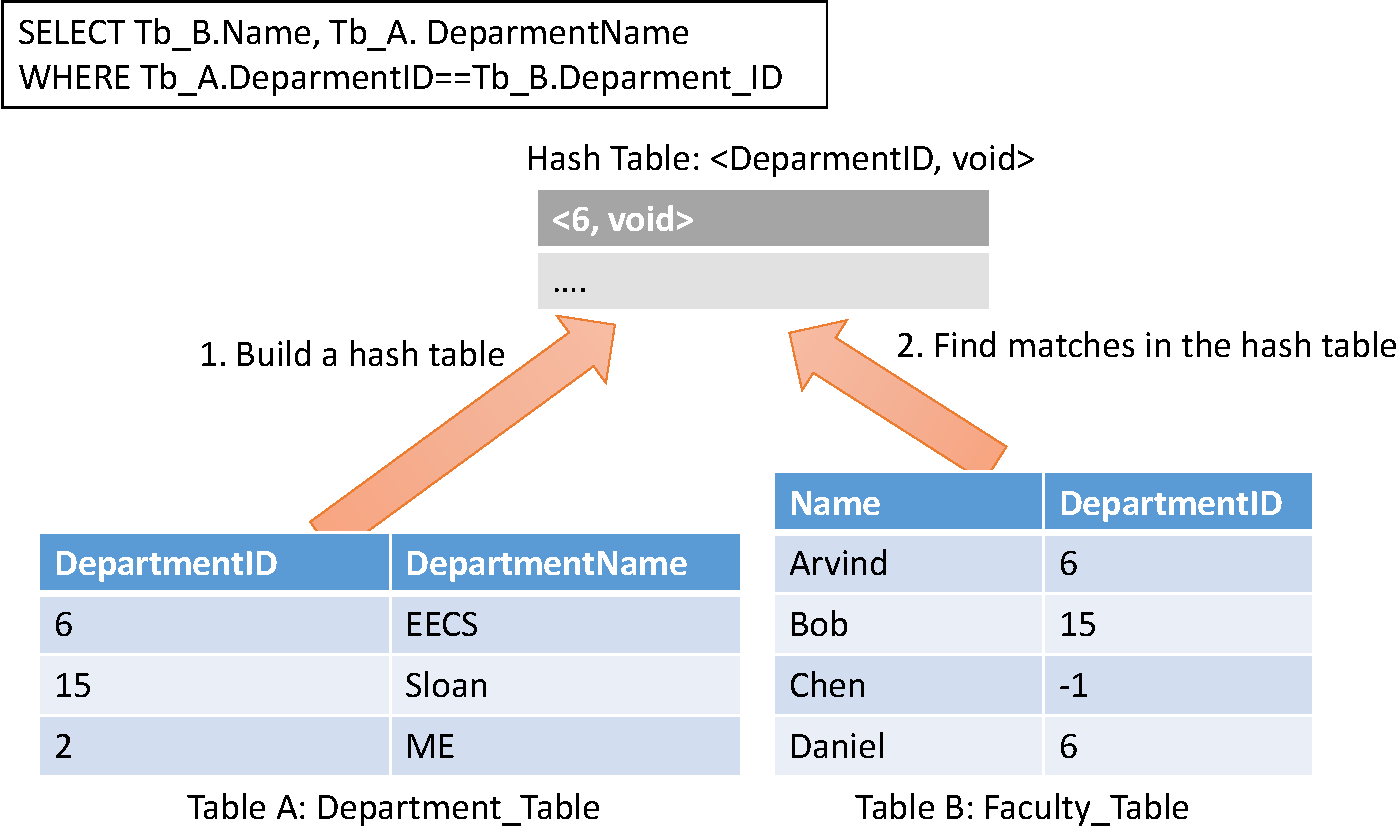
\includegraphics[width=\textwidth]{figures/hash-join-crop.pdf}
      \caption{Hash-join Operations without accelerators}
      \label{fig:hash-join}
  \end{subfigure}
  \begin{subfigure}[t]{0.48\textwidth}
    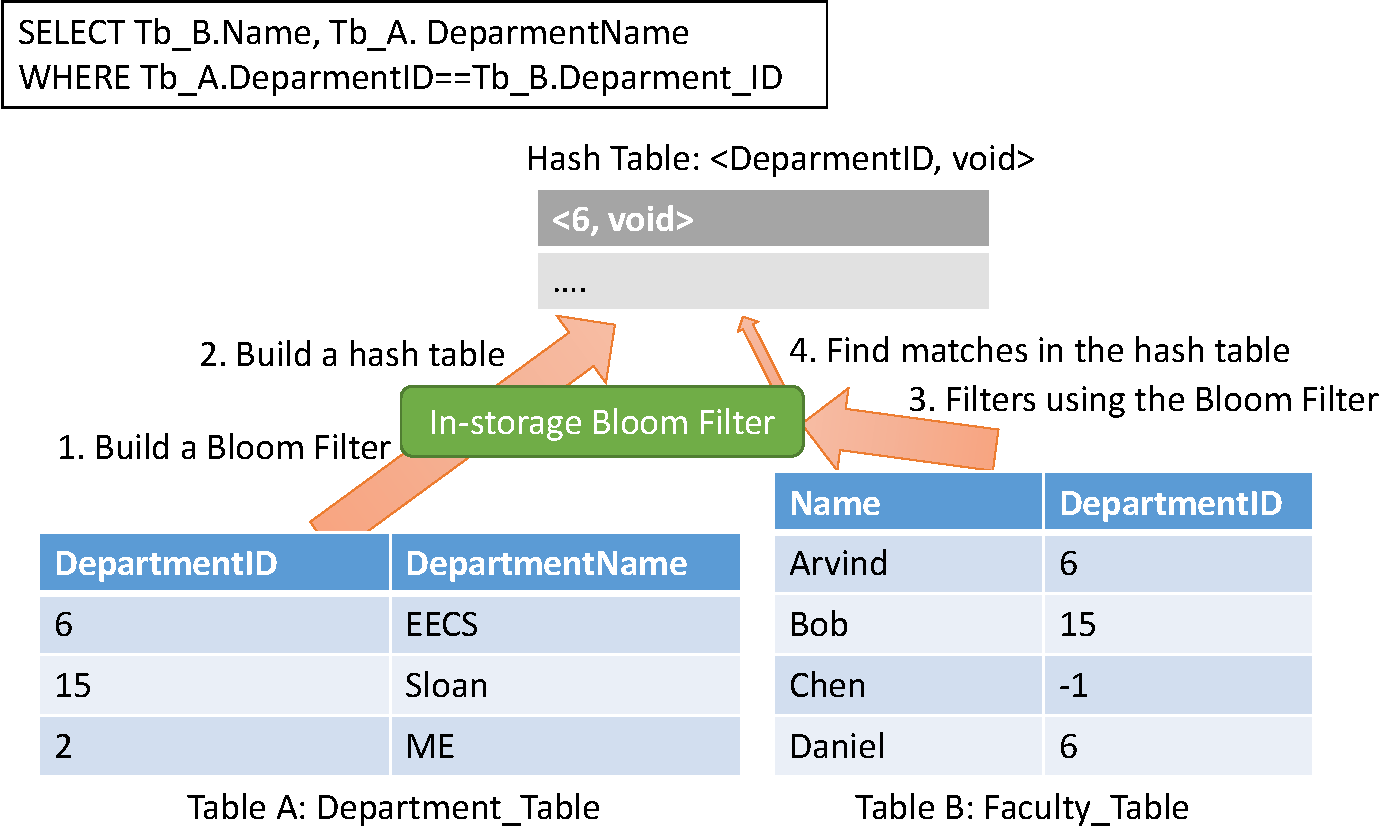
\includegraphics[width=\textwidth]{figures/filter-hash-join-crop.pdf}
    \caption{Accelerated Hash-join Operations with In-storage Bloom filter}
    \label{fig:filter-hash-join}
  \end{subfigure}
  \label{fig:try}
  \caption{Hash-join Operations}
\end{figure}

\subsection{TopK}

\topk sorts a table and only selects the first K rows according to the sorted attribute.
A traditional database would load the whole table from the storage, and executes an algorithm to select the top K rows (e.g., by sorting all the rows and choosing the first K). 
We observe that the IO traffic can be dramatically reduced by processing \topk operator in storage.
By offloading \topk operator to SSD, one can reduce the disk IO by from $\Omega(N)$ to $\Omega(K)$, where N the total number of rows of a table.

Our proposed FPGA-based implementation of \topk works as follows. 
The FPGA maintains a buffer of size K for the top K rows it has observed so far. 
For each batch of K rows loaded from the storage, the FPGA sorts in parallel the existing top K rows with the K incoming rows. 
The first K of the 2K sorted rows will remain as the new top K rows. 
The sorting of K rows can be implemented using a shorting network which can be parallelized and pipelined~\cite{fpga-sort}.

\subsection{Filter and Projection}

A filter operator will filter out database rows based on a predicate.
A projection operator will take the selected columns from database rows.
The computation of the filter and projection operators only requires one pass of the data and has little DRAM requirement.
Therefore, it is straightforward to implement these two operators on the near-data processor. 
Such designs have been extensively explored by previous work \cite{netezza,exadata,biscuit,sukhwani2012database,do2013query}.

\subsection{Group-By Aggregate}

Aggregate functions are typically used with \groupby database operations, where rows are grouped based on column values and each group of rows is summarized by applying the aggregate functions.
Instead of loading the whole table from the storage to the host node, an NDP-based \groupby implementation can perform the aggregate in the near-data processor, and thus greatly reduce the IO traffic. 
Previous work Ibex~\cite{ibex} has investigated how group-by aggregate works on FPGA.

\subsection{Index Probing}
\label{sec:index}

\indexing are intensively used in SQL queries to pinpoint row data locations when a certain column has a index.
Probing a b-tree index typically requires $\log{N}$ reads from SSDs, and the read latencies are additive.
If we offload  the index probing on in-storage processors, the latency of \indexing operations can be greatly reduced, because the slow storage network access is avoided.

\section{Evaluation Benchmarks}
\label{sec:eval}

We will conduct the performance evaluation on top of BlueDBM~\cite{bluedbm}, an FPGA-based NDP framework previously developed in our research group at MIT. On the host server, we plan to run a traditional relational database like MySQL, PostgreSQL, or SQLite. Both the storage-side FPGAs and the host-side database will be modified to implement the functionality of the operators. For performance evaluation, we will run synthetic queries, as well as a subset of queries from the TPC-H and TPC-DS workloads. Examples of such queries are shown below:

%some synthetic SQL queries with aggregate functions and join, as well as some queries from TPC-H, and TPC-DS.
%By comparing the same query on the same dataset running on the traditional relational database systems, such as MySQL and Postgres, we can illustrate the performance benefits of the new architecture with accelerators.
%Below are examples of SQL queries we plan to evaluate.

\begin{enumerate}

\item Query A: Synthetic query for evaluating aggregate accelerator 
\begin{verbatim}
SELECT department, years in company, SUM(salary) as sal sum
FROM employee GROUP BY department, years_in_company
\end{verbatim}

\item Query B: Modified Q14 of TPC-H for evaluating hash-join accelerator
\begin{verbatim}
SELECT sum(l_extendedprice * (1-l_discount)) as promo_revenue
FROM lineitem, part
WHERE l_partkey = p_partkey
and l_shipdate >= 1995-09-01 
and l_shipdate < 1995-10-01
\end{verbatim}

\item Query C: Q52 of TPC-DS for evaluating complex queries by both accelerators
\begin{verbatim}
SELECT dt.d_year, item.i_brand_id brand_id, item.i_brand brand,
SUM(ss_ext_sales_price) ext_price
FROM date_dim dt, store sales, item
WHERE dt.d date sk = store sales.ss sold date sk AND
store sales.ss item sk = item.i item sk AND
item.i manager id = 1 AND dt.d moy = 11 AND dt.d year = 2000
GROUP BY dt.d year, item.i brand, item.i brand id
ORDER BY dt.d year, ext price DESC, brand id
\end{verbatim}
\end{enumerate}

\bibliographystyle{abbrv}
\bibliography{reference}

\end{document}



